\chapter{Bayesian Networks}
\label{cha:bay_net}
All probabilistic inference (i.e. finding the probability of a variable of interest given what we know in terms of the other variables) and learning amount at repeated applications of the basic rules of probability (sum and product rules). Hence, in principle we do not need an additional framework to deal with relationships between variables. However, \textit{probabilistic graphical models} simplify a lot the management of multiple interconnected variables. Probabilistic graphical models are graphical representations of the \textit{qualitative} aspects of probability distributions allowing to:
\begin{itemize}
    \item visualize the structure of a probabilistic model (i.e. relationships between variables) in a simple and intuitive way
    \item discover properties of the model, such as conditional indipendencies, by visually inspecting the graph
    \item express complex computations for inference and learning in terms of graphical manipulations (e.g. information flows inside the graphical model)
    \item represent multiple probability distributions with the same graph, abstracting from their quantitative aspects (e.g. discrete vs continuous distributions). In a sense probabilistic graphical models are able to detach the qualitative aspects of probabilistic relationships from the quantitative aspects (e.g. the shape of the probability distribution which relates two different variables)
\end{itemize}

A \textit{Bayesian Network} (BN) structure ($\mathcal{G}$) is a \textit{directed graphical model}, so the connections between variables are characterized by a direction. Each node of the graph represents a random variable $x_i$. Each edge of the graph represents a direct dependency between two variables. Notice that if there is not an edge between two random variables $x_i, x_j$ we can not conclude that there is no probabilistic relationship between $x_i$ and $x_j$. Indeed, we have to take into account indirect relationships. In Figure \ref{fig:bayesianNetworkExample} it is reported an example of Bayesian Network. \newline

\textbf{Remark:} $\mathcal{G}$ has no cycles, i.e. it is a \textit{directed acyclic graph}.\newline

The structure encodes these independence assumptions:
\begin{equation}
    \mathcal{I}_l(\mathcal{G}) = \{\forall i \; x_i \perp \mathit{NonDescendants}_{x_i} | Parents_{x_i}\}
\end{equation}
each variable is independent ($\perp$) of its non-descendants given its parents.

\begin{figure}
    \centering
    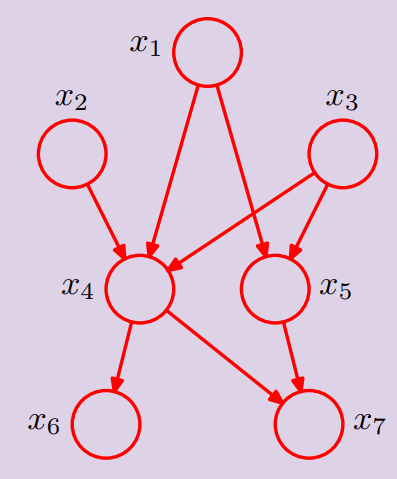
\includegraphics[width=0.5\textwidth]{images/bayesianNetworkExample.png}
    \caption{Bayesian Network example.}
    \label{fig:bayesianNetworkExample}
\end{figure}
The \textit{non-descendants} of a variable are the nodes which can not be reached following arrows from the variable. The subscript $l$ in $\mathcal{I}_l (\mathcal{G})$ stands for \textit{local} because, as discussed in the following, the model can also encode some global indipendences. \newline

Now we explain how to represent probabilistic relationships among a set of variables by means of a Bayesian Network.
\begin{itemize}
    \item Let $\mathcal{X}$ be a set of variables
    \item Let $p$ be a joint probability distribution over variables $\mathcal{X}$. Here we assume that $p$ is known, in practice we typically have to learn it from data
    \item Let $\mathcal{I}(p)$ be the set of independence assertions holding in $p$
    \item $\mathcal{G}$ is an \textit{independency map} (I-map) for $p$ if $p$ satisfies the local independences of $\mathcal{G}$:
    $$\mathcal{I}_l(\mathcal{G}) \subseteq \mathcal{I}(p)$$
    \textbf{Remark:} Note that given $\mathcal{I}_l(\mathcal{G}) \subseteq \mathcal{I}(p)$, the reverse is not necessarily true: there can be independences in $p$ that are not modelled by $\mathcal{G}$, perhaps we do not know them or the specific graphical model does not allow to encode them. Simmetrically, if we encode an independency in $\mathcal{G}$, this independecy should also hold in $p$.
\end{itemize}
Suppose we have to model a joint probability distribution $p(x_1, \hdots, x_m)$ among $m$ binary variables, we have to consider $2^m$ possible configurations which can soon become intractable. Our aim is to break down this joint probability into pieces. We say that $p$ \textit{factorizes} according to $\mathcal{G}$ if:
$$p(x_1, \hdots, x_m) = \prod_{i=1}^m p(x_i | \mathit{Pa}_{x_i})$$
where $\mathit{Pa}_{x_i}$ stands for the parents of $x_i$. Consider for example the Bayesian Network illustrated in Figure \ref{fig:bayesianNetworkExample}:
$$p(x_1, \hdots, x_7) = p(x_1)p(x_2)p(x_3)p(x_4|x_1,x_2,x_3)p(x_5|x_1,x_3)p(x_6|x_4)p(x_7|x_4,x_5)$$
Factorization is useful beacuse it breaks down a formula involving many variables into a product of formulas typically involving less values. In the example above, modeling $p(x_1,\hdots, x_7)$ as a single joint distribution, it would have required taking into consideration $2^7$ possible parameters (assuming only binary variables for simplicity), one for each possible configuration. On the other hand, the pieces on the left side of the equation involve significantly less paramaters:
\begin{itemize}
    \item $p(x_1),p(x_2),p(x_3)$ have 2 possible configurations
    \item $p(x_4|x_1,x_2,x_3)$ has $2^4$ possible configurations beacause it involves 4 variables
    \item $p(x_5|x_1,x_3), p(x_7|x_4,x_5)$ have $2^3$ possible configurations
    \item $p(x_6|x_4)$ has $2^4$ possible configurations
\end{itemize}
The order of complexity is around $2^4$ against $2^7$. \newline

This important result about factorization holds:
\begin{itemize}
    \item If $\mathcal{G}$ is an I-map for $p$, then $p$ factorizes according to $\mathcal{G}$
    \item If $p$ factorizes according to $\mathcal{G}$, then $\mathcal{G}$ is an I-map for $p$
\end{itemize}

The proof that this is the case follows: \newline

\textbf{I-map} $\Rightarrow$ \textbf{factorization}
\begin{enumerate}
    \item If $\mathcal{G}$ is an I-map for $p$, then $p$ satisfies (at least) these (local) independences:
    $$\{ \forall i \; x_i \perp \mathit{NonDescendants}_{x_i} | \mathit{Parents}_{x_i}\}$$
    
    \item Let us order variables in a \textit{topological order} relative to $\mathcal{G}$, i.e.:
    $$x_i \rightarrow x_j \Rightarrow i<j$$
    The variables in the Bayesian Network in Figure \ref{fig:bayesianNetworkExample} are already ordered topologically.
    
    \item Let us decompose the joint probability using the chain rule as:
    \begin{align*}
        p(x_1, \hdots, x_m) &= p(x_m | x_1, \hdots, x_{m-1})P(x_1,\hdots,x_{m-1})\\
        &= \prod_{i=1}^m p(x_i | x_1, \hdots, x_{i-1})
    \end{align*}
    
    \item Since nodes are topologically ordered, in $p(x_m | x_1, \hdots, x_{m-1})$ $x_m$ is conditioned on non-descendants. Local indipendences imply that for each $x_i$, in calculating $p(x_i | x_1, \hdots, x_{i-1})$, the only non-descendants $x_j \in \{x_1, \hdots, x_{i-1}\}$ which are relevant are the parents of $x_i$:
    $$p(x_i | x_1, \hdots, x_{i-1}) = p(x_i | \mathit{Pa}_{x_i})$$
\end{enumerate}

\textbf{factorization} $\Rightarrow$ \textbf{I-map}
\begin{enumerate}
    \item If $p$ factorizes according to $\mathcal{G}$, the joint probability can be written as:
    $$p(x_1, \hdots, x_m) = \prod_{i=1}^m p(x_i | \mathit{Pa}_{x_i})$$
    
    \item Let us consider the last variable $x_m$ (repeat steps for the other variables). By the product (chain) and sum rules:
    $$p(x_m|x_1, \hdots, x_{m-1}) = \frac{p(x_1, \hdots, x_{m})}{p(x_1, \hdots, x_{m-1})} = \frac{p(x_1, \hdots, x_{m})}{\sum_{x_m} p(x_1, \hdots, x_{m}))}$$
    
    \item Applying factorization and isolating the only term containing $x_m$ (the other terms which do not contain $m$ are constant with respect to the summation and can be taken out from the summation) we get:
    
    \begin{align*}
        \frac{p(x_1, \hdots, x_{m})}{\sum_{x_m} p(x_1, \hdots, x_{m}))} &= \frac{\prod_{i=1}^m p(x_i | \mathit{Pa}_{x_i})}{\sum_{x_m} \prod_{i=1}^m p(x_i | \mathit{Pa}_{x_i})} \\
        &= \frac{p(x_m | \mathit{Pa}_{x_m}) \cancel{\prod_{i=1}^{m-1} p(x_i|\mathit{Pa}_{x_i})}}{\cancel{\prod_{i=1}^{m-1} p(x_i | \mathit{Pa}_{x_i})} \cancel{\sum_{x_m}p(x_m | \mathit{Pa}_{x_m})}}
    \end{align*}
    
    \textbf{Remark:} $\sum_{x_m}p(x_m | \mathit{Pa}_{x_m})=1$ since we are summing over all possible values of $x_m$.\\
    \textbf{Remark:} In $p(x_m | x_1, \hdots, x_{m-1})$ all the variables in $\{x_1, \hdots, x_{m-1}\}$ are necessarily non-descendants of $x_m$ since we have defined a topological order.\\
    At the end of the day, we can conclude that the probability of $x_m$ given the non-descendants is equal to the probability of $x_m$ given the parents.
    
    \item If this property holds for $x_m$, for the same reasoning the property must holds for all the other variables. In other words, following this procedure we recover the set of independences that define an I-map.
\end{enumerate}

At this point we can conclude: factorization $\Leftrightarrow$ I-map.

\defi{\textbf{Bayesian Network} \label{def:bayesian_network}\\
A \textit{Bayesian Network} is a pair ($\mathcal{G}, p$) where $p$ factorizes over $\mathcal{G}$ (which is a Bayesian network structure) and it is represented as a set of conditional probability distributions (cpd) associated with the nodes of $\mathcal{G}$ ($p(x_1 | \mathit{Pa}_{x_1}), p(x_1 | \mathit{Pa}_{x_1}), \hdots, p(x_m | \mathit{Pa}_{x_m})$).

$$p(x_1, \hdots, x_m) = \prod_{i=1}^m p(x_i | \mathit{Pa}_{x_i})$$
}

\section{Example of Bayesian Network: toy regulatory network}
They are given three genes such that:
\begin{itemize}
    \item genes A and B have independent prior probabilities
    \item gene C can be enhanced by both A and B (if A and B are active, i.e. they are producing proteins, then it is more probable that also C is active)
\end{itemize}
We can represent this probabilistic setting with a Bayesian network as illustrated in Figure \ref{fig:geneBayesian}.
For the sake of simplicity, we assume that the variables are binary (active or inactive). In the context of binary variables, the conditional probability distribution becomes a conditional probability table, i.e. for each possible value of the variables there is a probability value.
According to the structure of the network, the joint probability decomposes as:
$$P(A,B,C) = P(C | A,B) P(A) P(B)$$
Since A and B have no parents, we simply build the two tables as follows:
\begin{center}
\begin{tabular}{c|c|c} 
 \hline
 gene & value & P(value)\\ 
 \hline
 A & active & 0.3\\ 
 A & inactive & 0.7
\end{tabular}
\end{center}

\begin{center}
\begin{tabular}{c|c|c} 
 \hline
 gene & value & P(value)\\ 
 \hline
 B & active & 0.3\\ 
 B & inactive & 0.7
\end{tabular}
\end{center}

On the other hand, mapping $P(C|A,B)$ is slightly more difficult. The conditional probability table has indeed 3 variables. The table is illustrated in Figure \ref{fig:geneBayesian_tableC}.\\
\textbf{Remark:} of course the columns of the conditional probability table proposed in Figure \ref{fig:geneBayesian_tableC} sum to one.

\begin{figure}
    \centering
    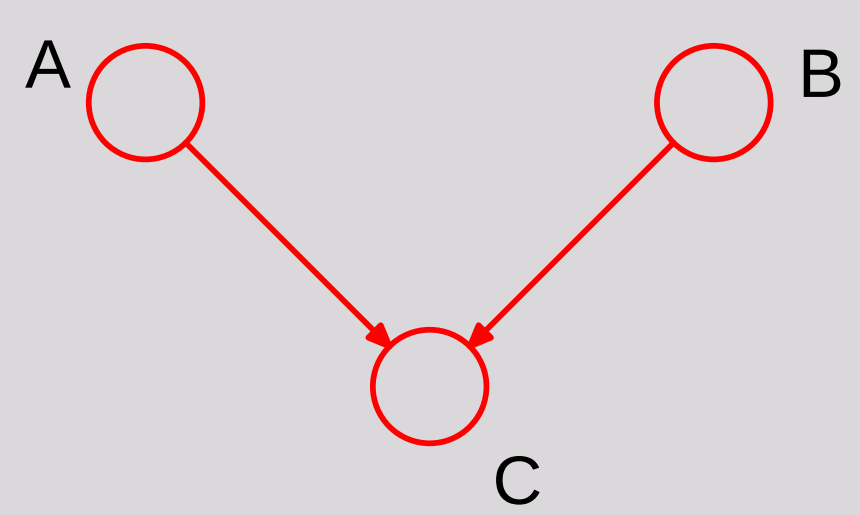
\includegraphics[width=0.5\textwidth]{images/geneBayesian.png}
    \caption{Toy regulatory network.}
    \label{fig:geneBayesian}
\end{figure}

\begin{figure}
    \centering
    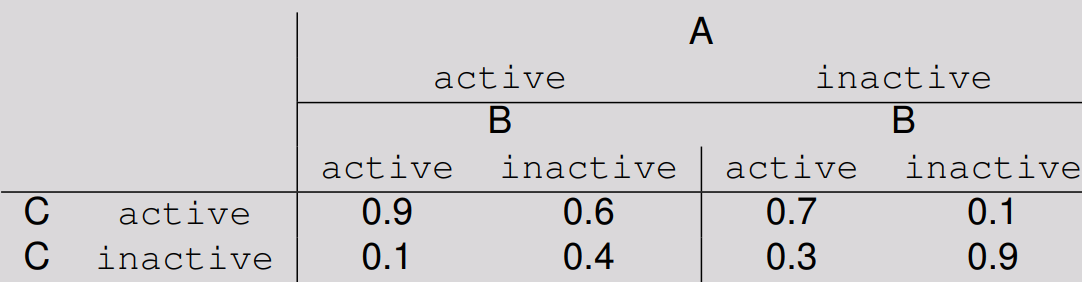
\includegraphics[width=\textwidth]{images/tabellaCGenes.png}
    \caption{Conditional probability table of gene C in the toy regulatory network proposed in Figure \ref{fig:geneBayesian}.}
    \label{fig:geneBayesian_tableC}
\end{figure}

\section{Conditional independence}
A graphical model is a way to make independences assumptions explicit in the structure of the model. \newline

Two variables $a,b$ are independent (written $a \perp b | \emptyset$) if:
\begin{equation}
    p(a,b) = p(a)p(b)
\end{equation}

Two variables $a,b$ are conditionally independent given $c$ (written $a \perp b | c$) if:
\begin{equation}
    \label{conditional_independence}
    p(a,b | c) = p(a|c) p(b|c)
\end{equation}

Independence assumptions can be verified by repeated applications of sum and product rules in order to see whether relations like \ref{conditional_independence} are actually true. However, doing these kind of mathematical derivations can become tedious. Whereas, with a graphical model which encodes the probability independences which we assume the distribution has, the procedure becomes simplier. Graphical models allow to directly verify independence assumptions through the \textit{d-separation} criterion.

\subsection{d-separation}
In order to introduce the process of d-separation, we start analyzing the base cases. The first relevant base case involves three variables. Indeed, the two variables case is trivial, since either the two variables are linked together and so they are related or there is no connection between the two variables and so they are not related. In a similar manner, also the case with three variables illustrated in Figure \ref{fig:trivialDSeparationThreeVariable} is trivial since each variable is related (i.e. there is a link) to the others. As a consequence everybody is dependent with respect to everybody else. There is nothing non-trivial to find out. The non-trivial case is when not all the three variables are connected to all the others (e.g. one link is missing). An example is illustrated in Figure \ref{fig:nonTrivialThreeVars}.

\begin{figure}
    \centering
    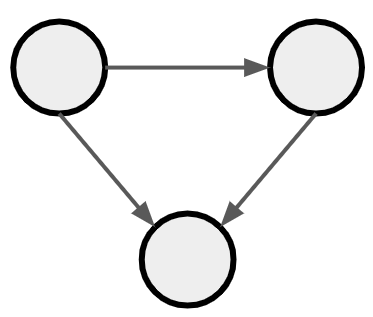
\includegraphics[width=0.5\textwidth]{images/exmpleTrivialThreeVariables.png}
    \caption{In this case although three variables are involved, verifying independency assumptions is trivial since each variable is related to the others.}
    \label{fig:trivialDSeparationThreeVariable}
\end{figure}

\begin{figure}
    \centering
    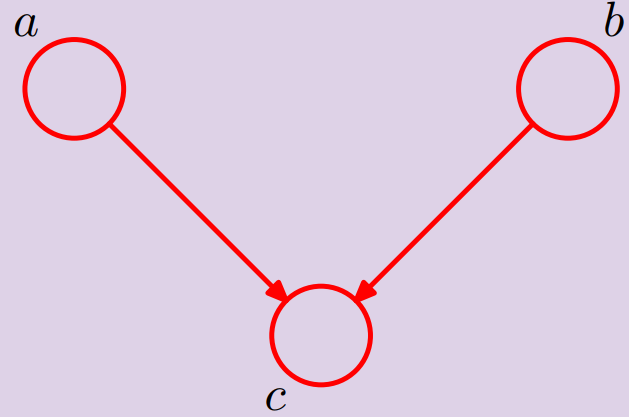
\includegraphics[width=0.5\textwidth]{images/nonTrivialThreeVars.png}
    \caption{In this case the independences among the three variables are not trivial.}
    \label{fig:nonTrivialThreeVars}
\end{figure}

In the following we discuss about the possible non trivial configurations of three variables. For consistency, we assume that the variable in the middle is identified with \textit{c}, while the variable on the left and the variable on the right are named \textit{a} and \textit{b} respectively.

\subsubsection{Tail-to-tail}
An example of this configuration is illustrated in Figure \ref{fig:tail-to-tail}.\\
The pattern is called \textit{tail-to-tail} because the central node \textit{c} is connected to the other variables by means of the tails of the two arrows.\\
Looking at the structure in Figure \ref{fig:tail-to-tail}, the joint probability distribution is:
$$p(a,b,c) = p(a|c)p(b|c)p(c)$$
At this point, our purpose is to understand whether $a$ and $b$ are independent ($a \perp b | \emptyset$) or not ($a \top\!\!\!\!\top b | \emptyset$). $a$ and $b$ are independent if:
$$p(a,b) = p(a)p(b)$$
Given $p(a,b,c)$ we get:
$$p(a,b) = \sum_c p(a,b,c)$$
According to the structure in Figure \ref{fig:tail-to-tail}, we can write:
$$p(a,b) = \sum_c p(a|c)p(b|c)p(c)$$

Actually, this formula does not simplify into $p(a)p(b)$:
$$p(a,b) = \sum_c p(a|c)p(b|c)p(c) \neq p(a)p(b)$$
as a result $a$ and $b$ are \textbf{not independent}. \newline
However, $a$ and $b$ are \textbf{conditionally independent given} $c$ (Figure \ref{fig:selectedTailToTail}):
\begin{equation*}
p(a,b|c) = \frac{p(a,b,c)}{p(c)} = \frac{p(a|c)p(b|c)p(c)}{p(c)} = p(a|c)p(b|c)
\end{equation*}

In other words, once $c$ is observed, $a$ and $b$ become independent. \newline

\textbf{Example 1:}
\begin{itemize}
    \item $a=$Bike
    \item $b=$Bus delay
    \item $c=$Rain
\end{itemize}

\textbf{Example 2:}
\begin{itemize}
    \item $a=$Cough
    \item $b=$Temperature
    \item $c=$Covid
\end{itemize}

\begin{figure}
\centering
\begin{subfigure}[t]{0.49\textwidth}
\centering
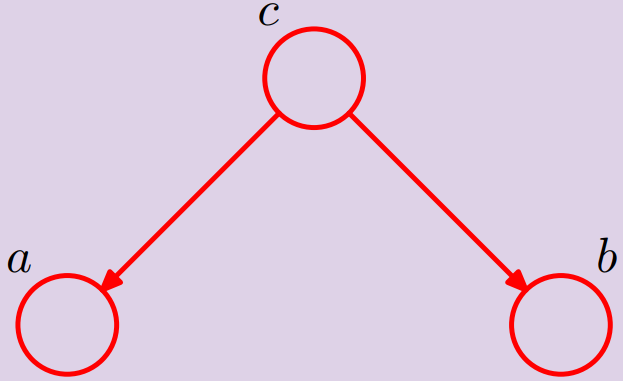
\includegraphics[width=\linewidth]{images/tailtToTail1.png} 
\caption{$a$ and $b$ are not independent.}
\label{fig:unSelectedTailToTail}
\end{subfigure}
\hfill
\begin{subfigure}[t]{0.49\textwidth}
\centering
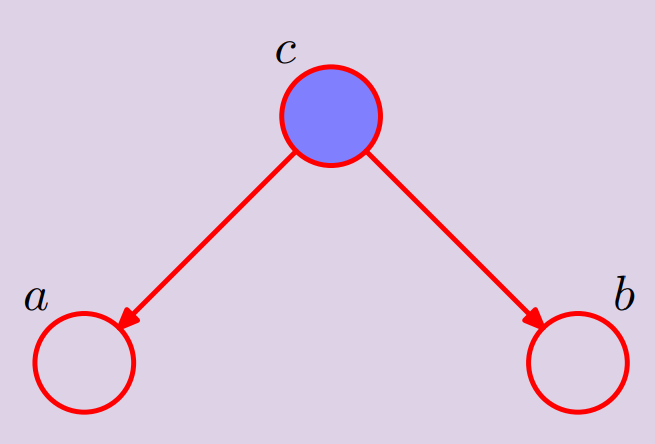
\includegraphics[width=\linewidth]{images/tailtToTailSelected.png}
\caption{$a$ and $b$ are conditionally independent given $c$.}
\label{fig:selectedTailToTail}
\end{subfigure}

\caption{Tail-to-tail}
\label{fig:tail-to-tail}
\end{figure}

\subsubsection{Head-to-tail}
In this case node $c$ is in the middle of a chain, Figure \ref{fig:head-to-tail}. Similarly to the previous case, this configuration is called \textit{head-to-tail} because variable $c$ is connected to $a$ and $b$ by means of the head of an arrow and a tail of another arrow. \newline

\textbf{Remark:} head-to-tail and tail-to-head are the same configuration because the labels $a$, $b$, $c$ are arbitrary. The only thing which matters is the chain that characterizes the structure. \newline

The joint probability $p(a,b,c)$ decomposes as follows:
$$p(a,b,c) = p(b|c)p(c|a)p(a)$$
We use this result to compute $p(a,b)$:
$$p(a,b) = \sum_c p(a,b,c) = p(a) \sum_c p(b|c)p(c|a)$$
There is no way applying probability rules to satisfy the equality $p(a) \sum_c p(b|c)p(c|a) = p(a)p(b)$. Given this, we can conclude that $a$ and $b$ are \textbf{not independent}:
$$p(a,b) = \sum_c p(b|c)p(c|a) \neq p(a)p(b)$$
On the other hand $a$ and $b$ are \textbf{conditionally independent given} $c$:
$$p(a,b | c) = \frac{p(a,b,c)}{p(c)} = \frac{p(b|c)p(c|a)p(a)}{p(c)}$$
Applying the Bayes rule we notice that:
$$\frac{p(c|a)p(a)}{p(c)} = p(a|c)$$
So:
$$p(a,b | c) = \frac{p(b|c)p(c|a)p(a)}{p(c)} = p(b|c)p(a|c)$$
Intuitively, if you have already observed the effects of a certain cause, you don't really care about the cause anymore in order to update the probability of the consequence. \newline

\textbf{Example:}
\begin{itemize}
    \item $a=$Cloudy
    \item $b=$Rainy
    \item $c=$Get wet
\end{itemize}
Assume that a student of the DISI department of the University of Trento named Giovanni Valer wakes up and notices that it's a cloudy day. He realizes that, if he goes to the university by bike, he could get wet. Indeed, since it is cloudy, it could rain. The fact that it is cloudy influences the chance of getting wet (causality reasoning).\\
Suppose not that Giovanni wakes up and it is raining but at the same time there is the sun. Even if it is not cloudy, Giovanni gets wet if he travels by bike to the university. Evidently, given that it is raining, the fact that it is not cloudy does not influence the probability of getting wet.

\begin{figure}
\centering
\begin{subfigure}[t]{0.49\textwidth}
\centering
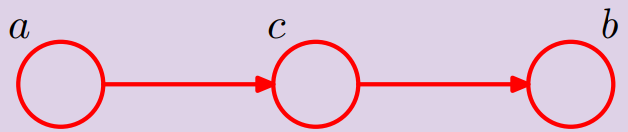
\includegraphics[width=\linewidth]{images/headToTail.png} 
\caption{$a$ and $b$ are not independent.}
\label{fig:unSelectedHeadToTail}
\end{subfigure}
\hfill
\begin{subfigure}[t]{0.49\textwidth}
\centering
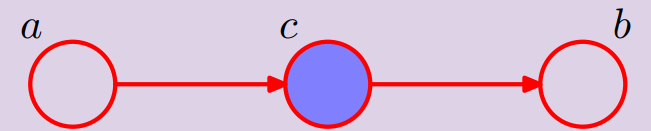
\includegraphics[width=\linewidth]{images/headToTailSelected.png}
\caption{$a$ and $b$ are conditionally independent given $c$.}
\label{fig:selectedHeadToTail}
\end{subfigure}

\caption{Head-to-tail}
\label{fig:head-to-tail}
\end{figure}

\subsubsection{Head-to-Head}
For the same reasons of the previous cases, the structure exemplified in Figure \ref{fig:head-to-head} is called \textit{head-to-head}. In this case the joint distribution decomposes as:
$$p(a,b,c) = p(c|a,b)p(a)p(b)$$
Calculating $p(a,b)$ summing over $c$ we notice that $p(a)$ and $p(b)$ can be extracted from the summation since they do not depend on $c$. Moreover, $\sum_c p(c|a,b) = 1$:
$$p(a,b) = \sum_c p(c|a,b) p(a) p(b) = p(a)p(b)$$

Therefore, we can conclude that $a$ and $b$ are \textbf{independent}. \newline

In this case we are not able to simplify $p(a,b|c)$ in order to verify the equality $p(a,b|c) = p(a|c)p(b|c)$. Actually, $a$ and $b$ are \textbf{not conditionally independent given} $c$:
$$p(a,b|c) = \frac{p(c|a,b)p(a)p(b)}{p(c)} \neq p(a|c)p(b|c)$$

Intuitively in this case $a$ and $b$ are competing causes of the effect $c$. At the beginning $a$ and $b$ are independent causes, but once the effect $c$ is observed they compete for the explanation. As a result, observing the result of one of them, reduces the probability of the other. This situation is usually referred to as \textit{explaining away effect}. \newline

\textbf{Example:}
\begin{itemize}
    \item $a=$Burglar
    \item $b=$Earthquake
    \item $c=$Alarm
\end{itemize}
Burglar and earthquake can be both possible causes for the alarm to ring. Of course, the burglar can decide to steal something from the house of Giovanni Valer regardless of the probability of an earthquake.\\
However, if the alarm rings Giovanni immediately thinks about a burglar. But if there is an earthquake in that moment, then the probability of a burglar in the mind of Giovanni decreases to 0.

\begin{figure}
\centering
\begin{subfigure}[t]{0.49\textwidth}
\centering
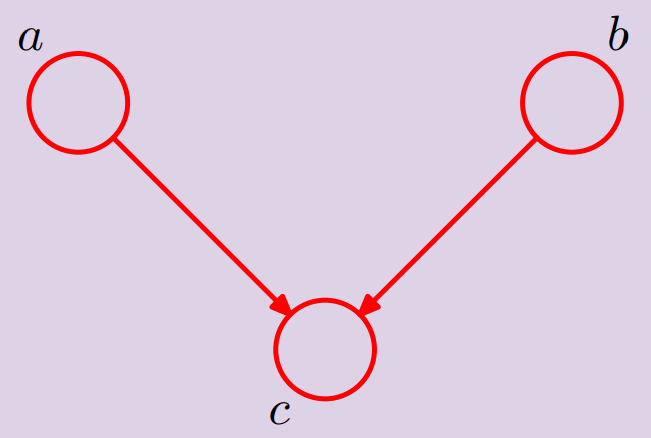
\includegraphics[width=\linewidth]{images/headToHead.png} 
\caption{$a$ and $b$ are independent.}
\label{fig:unSelectedHeadToHead}
\end{subfigure}
\hfill
\begin{subfigure}[t]{0.49\textwidth}
\centering
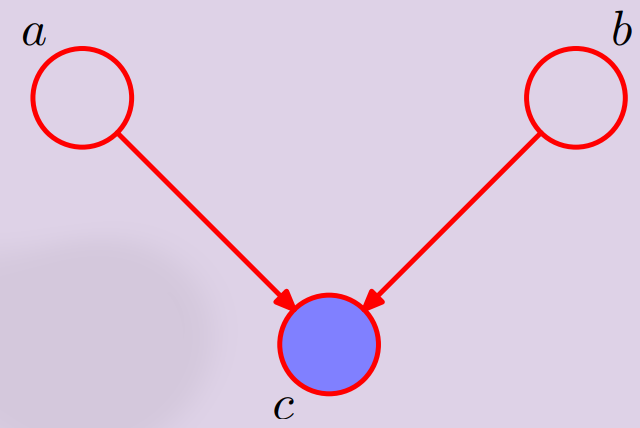
\includegraphics[width=\linewidth]{images/headToHeadSelected.png}
\caption{$a$ and $b$ are not conditionally independent given $c$.}
\label{fig:selectedHeadToHead}
\end{subfigure}

\caption{Head-to-head}
\label{fig:head-to-head}
\end{figure}

\begin{figure}
    \centering
    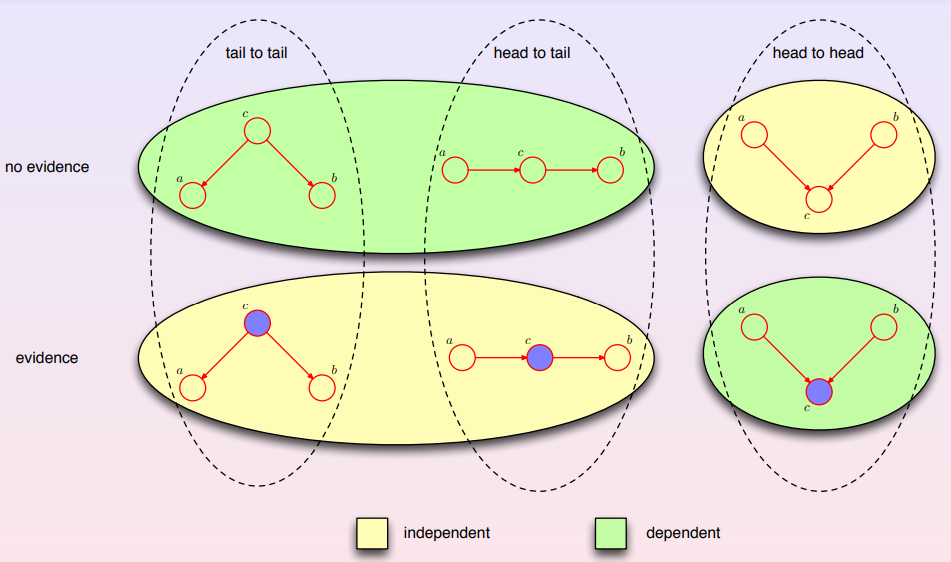
\includegraphics[width=\textwidth]{images/dSeparationSummary.png}
    \caption{d-separation: basic rules summary.}
    \label{fig:basicRulesSummary}
\end{figure}

\subsubsection{Example of head-to-head connection}
In this example we take into consideration a fuel system in a car. Our problem setting studies three random binary variables:
\begin{itemize}
    \item \textit{Battery}[B]: either charged (B=1) or flat (B=0)
    \item \textit{Fuel tank}[F]: either full (F=1) or empty (F=0)
    \item \textit{Electric fuel gauge}[G]: it indicates either full tank (G=1) or empty tank (G=0) 
\end{itemize}
The probabilistic dependences among these variables are represented by the Bayesian Network in Figure \ref{fig:fuelExample}. \newline

\textbf{Conditional probability tables (CPT)}
\begin{itemize}
    \item Battery and tank have independent prior probabilities:
    $$P(B=1) = 0.9$$
    $$P(F=1) = 0.9$$
    \item The fuel gauge is conditioned on both (unreliable):
    $$P(G=1 | B=1, F=1) = 0.8$$
    $$P(G=1 | B=0, F=1) = 0.2$$
    $$P(G=1 | B=1, F=0) = 0.2$$
    $$P(G=1 | B=0, F=0) = 0.1$$
\end{itemize}

\textbf{Probability reasoning} \newline

In this case the joint probability decomposes as follows:
$$P(F,G,B) = P(G | B,F)P(B)P(F)$$

Suppose that we are interesting in reasoning about the probability of empty tank.
\begin{itemize}
    \item The prior probability, without observing anything is:
    $$P(F=0) = 1 - P(F=1) = 0.1$$
    
    \item The posterior after observing empty fuel gauge (Figure \ref{fig:fuelExampleSelected}) is different:
    
    \begin{align*}
    P(F=0 | G=0) = \\
    &=\frac{P(G=0 | F=0) P(F=0)}{P(G=0)} =\\
    &=\frac{\sum_B [P(G=0,B | F=0)] P(F=0)}{P(G=0)} =\\
    &=\frac{\sum_B [P(G=0 | F=0, B) P(B|F=0)] P(F=0)}{P(G=0)}
    \end{align*}

    $F$ is not a descendant of $B$, as a result $P(B|F=0) = P(B)$. $B$ is independent with respect to its non descendants given the parents and $B$ has no parents.
    
    \begin{align*}
    P(F=0 | G=0) = \\
    &=\frac{\sum_B [P(G=0 | F=0, B) P(B|F=0)] P(F=0)}{P(G=0)} =\\
    &=\frac{\sum_B [P(G=0 | F=0, B) P(B)] P(F=0)}{P(G=0)}
    \end{align*}
    
    Now, we compute the denominator:
    \begin{align*}
    P(G=0) =\\
    &=\sum_{B \in \{0,1\}} \sum_{F \in \{0,1\}} P(G=0, B, F) =\\
    &= \sum_{B \in \{0,1\}} \sum_{F \in \{0,1\}} P(G=0 | B, F)P(B,F) = \\
    &= \sum_{B \in \{0,1\}} \sum_{F \in \{0,1\}} P(G=0 | B, F) P(F|B) P(B)
    \end{align*}
    Given the network, $F$ is independent with respect to its non descendants given its parents and $F$ has no parents.
    \begin{align*}
        P(G=0) =\\
        &= \sum_{B \in \{0,1\}} \sum_{F \in \{0,1\}} P(G=0 | B, F) P(F|B) P(B)\\
        &=\sum_{B \in \{0,1\}} \sum_{F \in \{0,1\}} P(G=0 | B, F)P(B)P(F)
    \end{align*}
    
    At the end of the day:
    \begin{align*}
    P(F=0 | G=0) =\\
    &=\frac{\sum_B [P(G=0 | F=0, B) P(B)] P(F=0)}{P(G=0)} =\\
    &=\frac{\sum_B [P(G=0 | F=0, B) P(B)] P(F=0)}{\sum_{B \in \{0,1\}} \sum_{F \in \{0,1\}} P(G=0 | B, F)P(B)P(F)} \simeq 0.257
    \end{align*}
    
\end{itemize}

The probability that the tank is empty increases from observing that the fuel gauge reads empty (not as much as expected because a strong prior and unreliable gauge). \newline

\textbf{Remark:} In real world applications, we typically observe the effects rather than the causes (e.g. we observe symptoms, not the pathology). We have to apply probability rules and in particular the Bayes theorem in order to reason about the probability of the causes. This is why this structures are named Bayesian Networks. \newline

\begin{figure}
\centering
\begin{subfigure}[t]{0.32\textwidth}
\centering
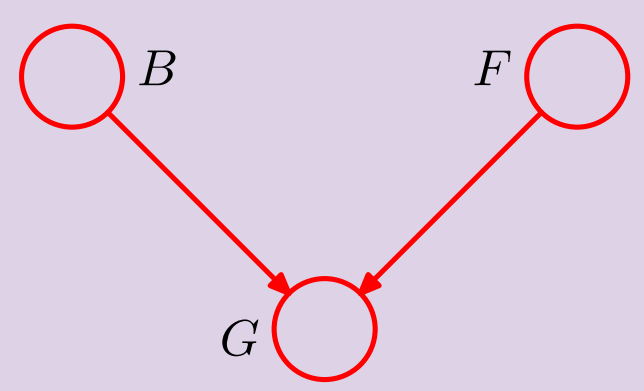
\includegraphics[width=\textwidth]{images/fuelExample.png}
\caption{Example of head-to-head connection.}
\label{fig:fuelExample}
\end{subfigure}
\hfill
\begin{subfigure}[t]{0.32\textwidth}
\centering
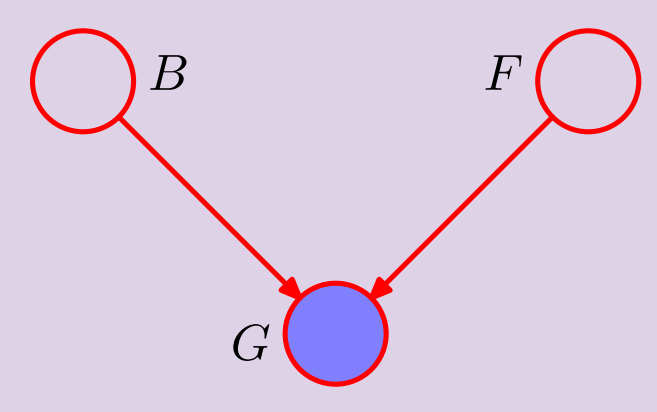
\includegraphics[width=\linewidth]{images/fuelExampleSelected.png}
\caption{The probability that the tank is empty increases from observing that the fuel
gauge reads empty.}
\label{fig:fuelExampleSelected}
\end{subfigure}
\hfill
\begin{subfigure}[t]{0.32\textwidth}
\centering
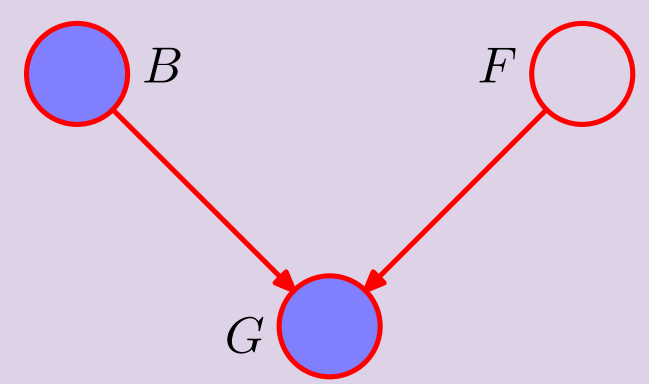
\includegraphics[width=\linewidth]{images/fuelExamplePart2.png}
\caption{The probability that the tank is empty decreases after observing that the battery is also flat.}
\label{fig:fuelExampleSelectedPart2}
\end{subfigure}

\caption{Head-to-head}
\label{fig:head-to-head-example}
\end{figure}

Suppose that now, we are interesting in the posterior probability after observing that the battery is also flat (Figure \ref{fig:fuelExampleSelectedPart2}).

\begin{align*}
P(F=0 | G=0, B=0) = \\
&=\frac{P(G=0|F=0,B=0)P(F=0|B=0)}{P(G=0|B=0) \simeq 0.111}
\end{align*}

From this we understand that $F$ and $B$ are related once $G$ is known. If they were unrelated, knowing something about $B$ would not change the probability value. On the contrary, the probability that the tank is empty decreases after observing that the battery is also flat. The battery condition \textit{explains away} the observation that the fuel gauge reads empty. The probability is sill greater than the prior one, because the fuel gauge observation still gives some evidence in favour of an empty tank.

\subsubsection{d-separation in networks with more than three variables}
Naturally, it is interesting to study more complex configurations involving more than three random variables. \newline

\textbf{General Head-to-head}
\begin{itemize}
    \item Let a descendant of a node $x$ be any node which can be reached from $x$ with a path following the direction of the arrows.
    \item A head-to-head node $c$ unblocks the dependency path between its parents if either itself or any of its descendants receives evidence.
\end{itemize}

Consider the example in Figure \ref{fig:generalHeadToHead1}. As we explained above, $A$ and $B$ are independent in principle. However, once $C$ receives evidence, then $A$ and $B$ are dependent one with respect to the other. Analogously, in Figure \ref{fig:generalHeadToHead2} variables $A$ and $B$ are initially independent, but when $D$, which is a child of $C$, is observed, then $A$ and $B$ becomes mutually dependent. For instance, the four variables could represent the following events:
\begin{itemize}
    \item $A=$ burglar
    \item $B=$ earthquake
    \item $C=$ alarm
    \item $D=$ phone call from the alarm company
\end{itemize}
If Giovanni Valer is not at home but he receives a phone call from the alarm company he immediately thinks about a burglar even if he does not hear the alarm. Evidently, burglar and earthquake both compete for an indirect effect. \newline

This rules is valid for every descendant, though probably the further the descendant the less influent is the indirect connection.

\begin{figure}
\centering
\begin{subfigure}[t]{0.49\textwidth}
\centering
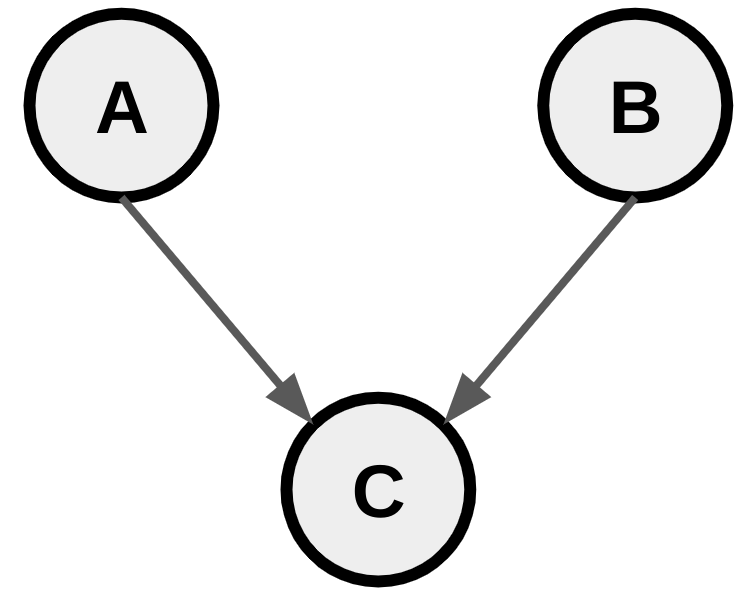
\includegraphics[width=\textwidth]{images/generalHeadToHead1.png}
\caption{Head-to-head connection among three random variables.}
\label{fig:generalHeadToHead1}
\end{subfigure}
\hfill
\begin{subfigure}[t]{0.49\textwidth}
\centering
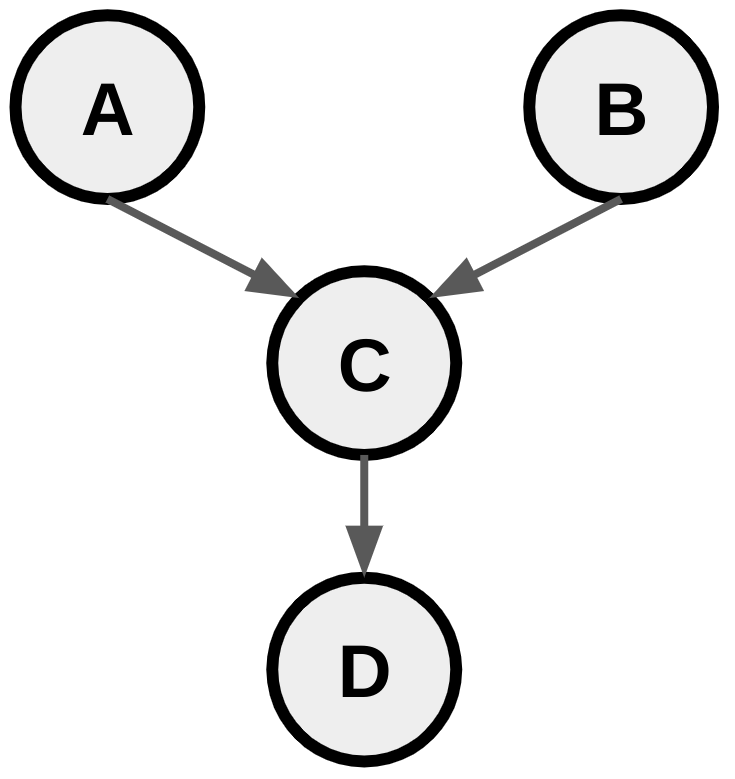
\includegraphics[width=\linewidth]{images/generalHeadToHead2.png}
\caption{Head-to-head connection among more than three random variables.}
\label{fig:generalHeadToHead2}
\end{subfigure}

\caption{General Head-to-head}
\label{fig:generalHeadToHead}
\end{figure}

\subsubsection{General d-separation criterion}
Given a generic Bayesian network. Given $A,B,C$ arbitrary nonintersecting sets of nodes. The sets $A$ and $B$ are \textit{d-separated} by $C$ ($\mathit{dsep}(A;B|C)$) if all paths from any node in $A$ to any node in $B$ are \textit{blocked} (there is no information flow along the path). Actually, if there is no information flow between $A$ and $B$, then $A$ and $B$ are independent given $C$.\\
A path is blocked if it includes at least one node s.t. either:
\begin{itemize}
    \item the arrows on the path meet tail-to tail (Figure \ref{fig:selectedTailToTail}) or head-to-tail (Figure \ref{fig:selectedHeadToTail}) at the node and it is in $C$, or
    \item the arrows on the path meet head-to-head at the node and neither it nor any of its descendants is in $C$ (Figure \ref{fig:selectedHeadToHead}).
\end{itemize}

\defi{\textbf{d-separation implies conditional independence} \label{def:d-separation}\\
The sets $A$ and $B$ are independent given $C$ ($A \perp B | C$) if they are d-separated by $C$.
}

In a sense, we are using the basic rules in Figure \ref{fig:basicRulesSummary} as building blocks to define the more general d-separation principle. The basic rules allow to understand if individual paths are blocked somewhere. It is sufficient that a path is blocked in one place to be completely blocked. \newline

\textbf{Example of general d-separation 1}

In this second example we consider the Bayesian Network in Figure \ref{fig:exampleDSeparation1}. In this case nodes $a$ and $b$ are not d-separated by $c$:
\begin{itemize}
    \item Node $f$ is tail-to-tail and not observed.
    \item Node $e$ is head-to-head and its child $c$ is observed.
\end{itemize}

We can conclude that $a \top\!\!\!\!\top b | c$. In other words, there is information flow from $a$ to $b$. \newline

\begin{figure}
    \centering
    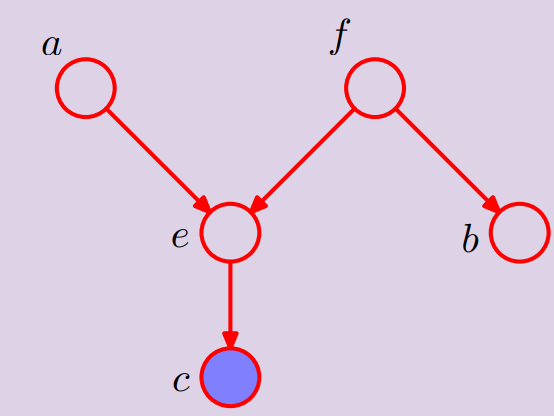
\includegraphics[width=0.5\textwidth]{images/exampleGeneralDSeparation1.png}
    \caption{Example of general d-separation. $a \top\!\!\!\!\top b | c$ }
    \label{fig:exampleDSeparation1}
\end{figure}

\textbf{Example of general d-separation 2} \newline
In this second example we consider the Bayesian Network in Figure \ref{fig:exampleDSeparation1.1}. In this case $a$ and $b$ are d-separated by $e$:
\begin{itemize}
    \item $e$ is head-to-head connected.
    \item $e$ is not observed.
    \item no children of $e$ are observed.
\end{itemize}

As a result there is no information flow via $e$. We can conclude that $\mathit{dsep}(A,B | \emptyset)$. \newline

\begin{figure}
    \centering
    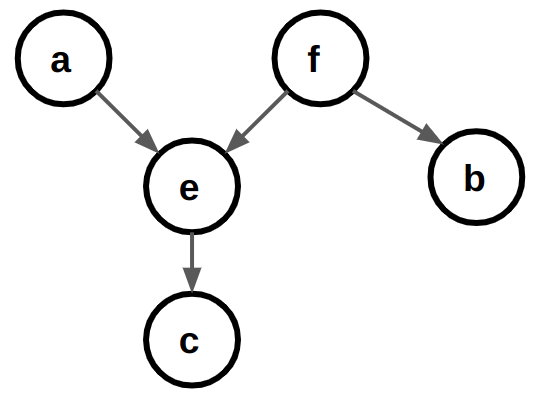
\includegraphics[width=0.5\textwidth]{images/exampleGeneralDSeparation1.1.png}
    \caption{Example of general d-separation. $a \perp b | c$ }
    \label{fig:exampleDSeparation1.1}
\end{figure}

\textbf{Example of general d-separation 3}

In this third example we consider the Bayesian Network in Figure \ref{fig:exampleDSeparation2}. In this case $a$ and $b$ are d-separated by $f$:
\begin{itemize}
    \item Node $f$ is tail-to-tail and observed.
\end{itemize}

In this case node $f$ blocks the flow of information. We can conclude that $a \perp b | f$. Intuitively, $a$ and $f$ are two possible causes for $b$. If $f$ is observed than the cause is already known. \newline

\begin{figure}
    \centering
    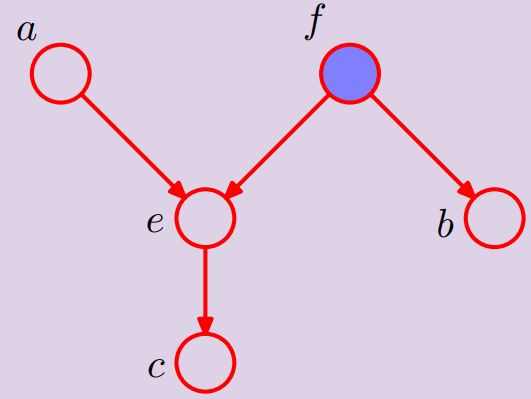
\includegraphics[width=0.5\textwidth]{images/exampleGeneralDSeparation2.png}
    \caption{Example of general d-separation. $a \perp b | c$ }
    \label{fig:exampleDSeparation2}
\end{figure}

\textbf{Example of general d-separation 4} \newline
In this fourth example, we consider the network in Figure \ref{fig:exampleDSeparation4} and we investigate if $A$ and $B$ are d-separated or not ($\mathit{dsep}(A,B|C)$). In order to answer to this question we have to examine all the possible paths between $A$ and $B$. In correspondence of $\alpha$ there is a head-to-head connection and node $\alpha$ is observed. Hence, we can conclude that information flows from $A$ to $B$ and the statement $\mathit{dsep}(A,B|C)$ is not true. \newline

\begin{figure}
    \centering
    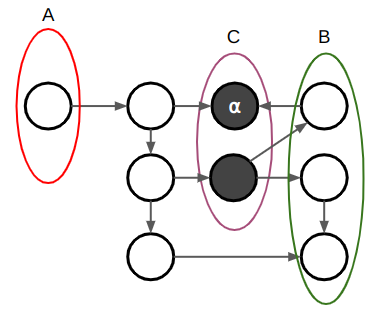
\includegraphics[width=0.5\textwidth]{images/exampleGeneralDSeparation3.png}
    \caption{Example of general d-separation. $A \top\!\!\!\!\top B | C$ }
    \label{fig:exampleDSeparation4}
\end{figure}

\textbf{Example of general d-separation 5} \newline
In this fifth example, we consider the network illustrate in Figure \ref{fig:exampleDSeparation5}. In this case the path 1-2-3-4 is blocked because in correspondence of node 3 there is a head-to-head connection but node 3 is not observed and it has no children. As a consequence we have to check other paths in order to understand whether or not $\mathit{dsep}(A,B|C)$. Moreover also paths 1-2-5-$\beta$-6 and 1-2-5-$\beta$-4 are blocked. However, along the chain 1-2-5-7-8 there are no observations. So along 1-2-5-7-8 information flows. We can conclude that $A$ and $B$ are not d-separated. \newline

\begin{figure}
    \centering
    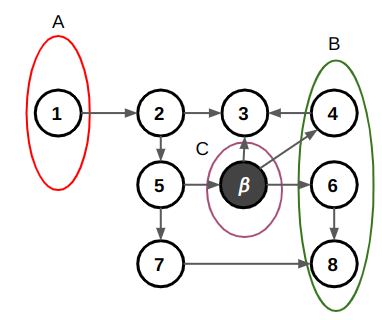
\includegraphics[width=0.5\textwidth]{images/exampleGeneralDSeparation4.png}
    \caption{Example of general d-separation. $A \top\!\!\!\!\top B | C$ }
    \label{fig:exampleDSeparation5}
\end{figure}

\textbf{Example of general d-separation 6} \newline
In this sixth example we consider the network illustrated in Figure \ref{fig:exampleDSeparation6}. Following the same reason as before, we understand that $A$ and $B$ are d-separated by $C$ this time.

\begin{figure}
    \centering
    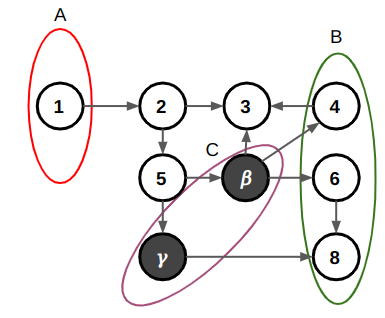
\includegraphics[width=0.5\textwidth]{images/exampleGeneralDSeparation5.png}
    \caption{Example of general d-separation. $A \perp B | C$ }
    \label{fig:exampleDSeparation6}
\end{figure}

\subsection{BN independences revisited}
\begin{itemize}
    \item A BN structure $\mathcal{G}$ encodes a set of \textit{local} independence assumptions:
    $$I_l(\mathcal{G}) = \{\forall i x_i \perp \mathit{NonDescendants}_{x_i}|\mathit{Parents}_{x_i}\}$$
    
    \item A BN structure $\mathcal{G}$ encodes a set of \textit{global} (Markov) independence assumptions:
    $$I(\mathcal{G}) = \{(A \perp B | C) : \mathit{dsep}(A;B|C)\}$$
\end{itemize}

\subsection{BN equivalence classes}
Quite different BN structures can actually encode the exact same set of independence assumptions. For example the three BNs in Figure \ref{fig:exampleIEquivalentBN} constitutes an equivalence class whose components encode the same independence assumptions. Figure \ref{fig:exampleIEquivalentBN2} represents the second independence class which encodes the opposite ($A$ and $B$ are not independent, they become independent when $C$ is observed) of the structures in Figure \ref{fig:exampleIEquivalentBN}. This concept can be generalized to arbitrary Bayesian Networks with more than three nodes. In general two BN structures (of course they have to be on the same set of nodes) $\mathcal{G}$ and $\mathcal{G}'$ are \textit{I-equivalent} if $I(G)=I(\mathcal{G}')$. Following this relation, the space of BN structures over $\mathcal{X}$ is partitioned into a set of mutually exclusive and exhaustive \textit{I-equivalence classes}.

\begin{figure}
\centering
\begin{subfigure}[t]{0.49\textwidth}
\centering
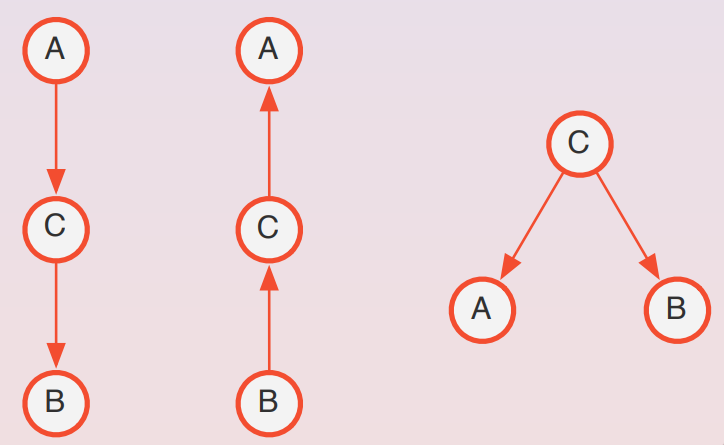
\includegraphics[width=\textwidth]{images/exampleIEquivalentBN.png}
\caption{The three BNs constitutes an equivalence class whose components encode the same independence assumptions.}
\label{fig:exampleIEquivalentBN}
\end{subfigure}
\hfill
\begin{subfigure}[t]{0.49\textwidth}
\centering
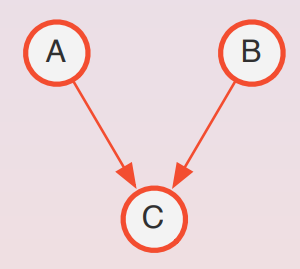
\includegraphics[width=0.7\linewidth]{images/exampleIEquivalentBN2.png}
\caption{A second independence class which encodes the opposite ($A$ and $B$ are not independent, they become independent when $C$ is observed) of the structures in Figure \ref{fig:exampleIEquivalentBN}.}

\label{fig:exampleIEquivalentBN2}
\end{subfigure}

\caption{BN equivalence classes}
\label{fig:BNequivalenceclasses}
\end{figure}

\section{I-maps vs distributions}
As explained above, for a structure $\mathcal{G}$ to be an I-map for $p$, it does not need to encode all its independences. As a consequence a fully connected graph is an I-map of any $p$i defined over its variables. Indeed, a fully connected graph does not encode any independency and so, for sure it does not encode an independency which is not in $p$. Obviously, a fully connected graph is not useful for our purposes.

\defi{\textbf{Minimal I-map} \label{def:minimalIMap}\\
A \textit{minimal I-map} for $p$ is an I-map $\mathcal{G}$ which can't be "reduced" into a $\mathcal{G}' \subset \mathcal{G}$ (by removing edges) that is also an I-map for $p$. In other words it is no more possible to remove edges from $\mathcal{G}$ without introducing independences which do not hold in $p$.
}

\textbf{Remark:} a minimal I-map for $p$ does not necessarily capture all the independences in $p$.

\defi{\textbf{Perfect Maps (P-maps)} \label{def:perfectMap}\\
A structure $\mathcal{G}$ is a \textit{perfect map} (P-map) for $p$ it captures all (and only) its independences:
$$I(\mathcal{G}) = I(p)$$
}

\textbf{Remark:} not all distributions have a P-map. Some cannot be modelled exactly by the BN formalism. In particular there are some independences which cannot be modelled by directed edges. \newline

There exists an algorithm for finding a P-map of a distribution which is exponential in the in-degree of the P-map. The algorithm returns an equivalence class of structures which are a perfect map rather than a single structure.

\section{Practical suggestions for building a Bayesian Network}
\label{sec::practicalSuggestions}
\begin{itemize}
    \item Get together with a domain expert.
    
    \item Define variables for entities that can be \textit{observed} (e.g. symptoms, age, weight) or that you can be interested in \textit{predicting} (e.g. pathology). Latent variables can also be sometimes useful. Latent variables are variables which we do not observe and we do not want to predict. However, they are mediators for what we need to predict. For instance, a certain pathology could depend on some groups of behaviours which could facilitate the prediction of the pathology.
    
    \item Try following \textit{causality} considerations in adding edges (edges which encode causalities are more interpretable and they tend to produce sparser networks).
    
    \item In defining probabilities for configurations (almost) never assign zero probabilities. Otherwise, every example with that configuration which we will observe in the future will have zero probability.
    
    \item It is usually difficult in real world applications to assign probabilities to certain variables configurations. As a result we typically refine or estimates these parameters using data. If data are available, use them to help in \textit{learning} parameters and structure of the network.
\end{itemize}